\documentclass[a4paper, 10pt, conference]{ieeeconf}

\overrideIEEEmargins                                      % Needed to meet printer requirements.

% See the \addtolength command later in the file to balance the column lengths
% on the last page of the document

\usepackage{graphicx} % for pdf, bitmapped graphics files
%\usepackage{epsfig}   % for postscript graphics files
%\usepackage{mathptmx} % assumes new font selection scheme installed
%\usepackage{times}    % assumes new font selection scheme installed
%\usepackage{amsmath}  % assumes amsmath package installed
%\usepackage{amssymb}  % assumes amsmath package installed

\title{ %\LARGE \bf
  Distributed Intelligent Systems: Course Project\\
  Swarm compactness maintenance using only local communication
}

\author{
  Morgan Bruhin (\texttt{morga.bruhin@epfl.com}) \\
  Merlin Nimier David (\texttt{merlin.nimier-david@epfl.com}) \\
  Krishna Raj Sapkota (\texttt{krishna.sapkota@epfl.com})
}

\begin{document}

\maketitle
\thispagestyle{empty}
\pagestyle{empty}

%%%%%%%%%%%%%%%%%%%%%%%%%%%%%%%%%%%%%%%%%%%%%%%%%%%%%%%%%%%%%%%%%%%%%%%%%%%%%%%%
\begin{abstract}
  Short, but concise description of your project and results.
  Here's how to reference articles from the bibliography: \cite{Nembrini02} and \cite{Winfield08}.
\end{abstract}

\section{Introduction}
  TODO: brief description of your project and why it is interesting (with citations)\\

  Define Swarm Robotics. Describe the Coherent Swarming problem.\\

  Present the Alpha algorithm (solution proposed by \cite{Nembrini02}). Present Beta algorithm.

  Define Multilevel modeling (3 levels). Explain the advantages / usage of macroscopic modeling. Present solution proposed by \cite{Winfield08}.

%%%%%%%%%%%%%%%%%%%%%%%%%%%%%%%%%%%%%%%%%%%%%%%%%%%%%%%%%%%%%%%%%%%%%%%%%%%%%%%%

\section{Experiments}
  TODO: what you did in your project\\

  \subsection{State machine}
  Present the controller's states. Explain the transitions. Explain the obstacle avoidance behavior (Braitenberg's controller).

  \subsection{Experimental setup}
  Webots software, arena. E-puck robot: which sensors, which abilities. Communication model (range and delays). No noise used on messages.\\

  \subsection{Experimental parameters}
  We summarize below the parameters used in our simulations.

  \begin{table}[h]
    \begin{center}
      \begin{tabular}{r|ll}
        \hline
        Parameter                  & Value               & Unit\\
        \hline
        Experiment duration        & $1000$              & seconds\\
        Number of agents           & $40$                & robots\\
        $\alpha$                   & $5$, $10$ and $15$  & neighbors\\
        $\beta$                    & $5$                 & neighbors\\
        Simulation timestep        & $64$                & milliseconds\\
        $T$ (communication period) & $20$                & timesteps\\
        $T_A$ (avoidance period)   & $5$                 & timesteps\\
        $T_C$ (coherence period)   & $80$                & timesteps\\
        Communication radius       & $0.7$               & meters\\
        \hline
      \end{tabular}
      \caption{Experimental parameters}
    \end{center}
  \end{table}

  \subsection{Implementation}
  Implemented in C in Webots. Automatic simulation logging at each communication step.\\

  \subsection{Macroscopic model}
  Implementation of the differential equations in Matlab.\\
  Then, calibration of the probabilities from the simulation's results.

\section{Results}
  TODO: what you discovered (you may want to include tables or plots here)\\

  \begin{figure}[h]
    \begin{center}
      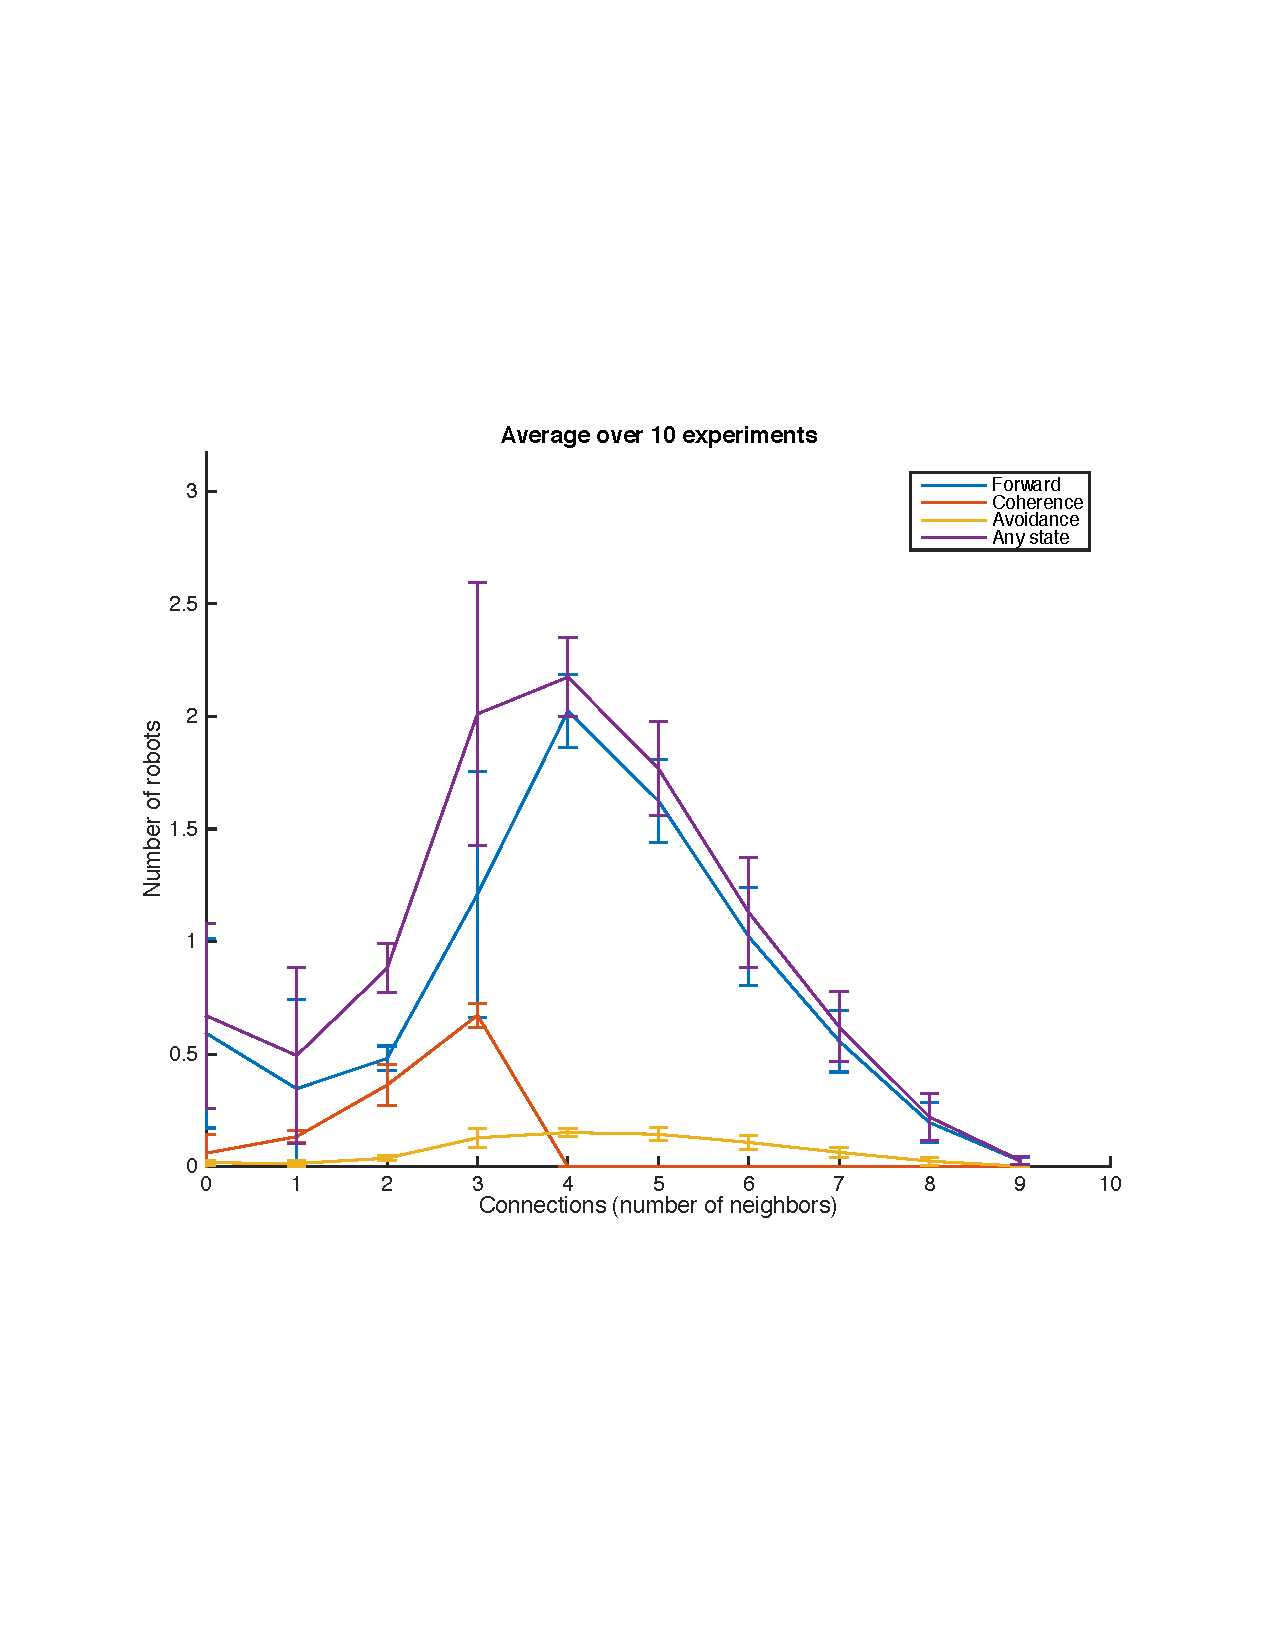
\includegraphics[width=8cm]{figures/simulation-10-alpha4.pdf}
      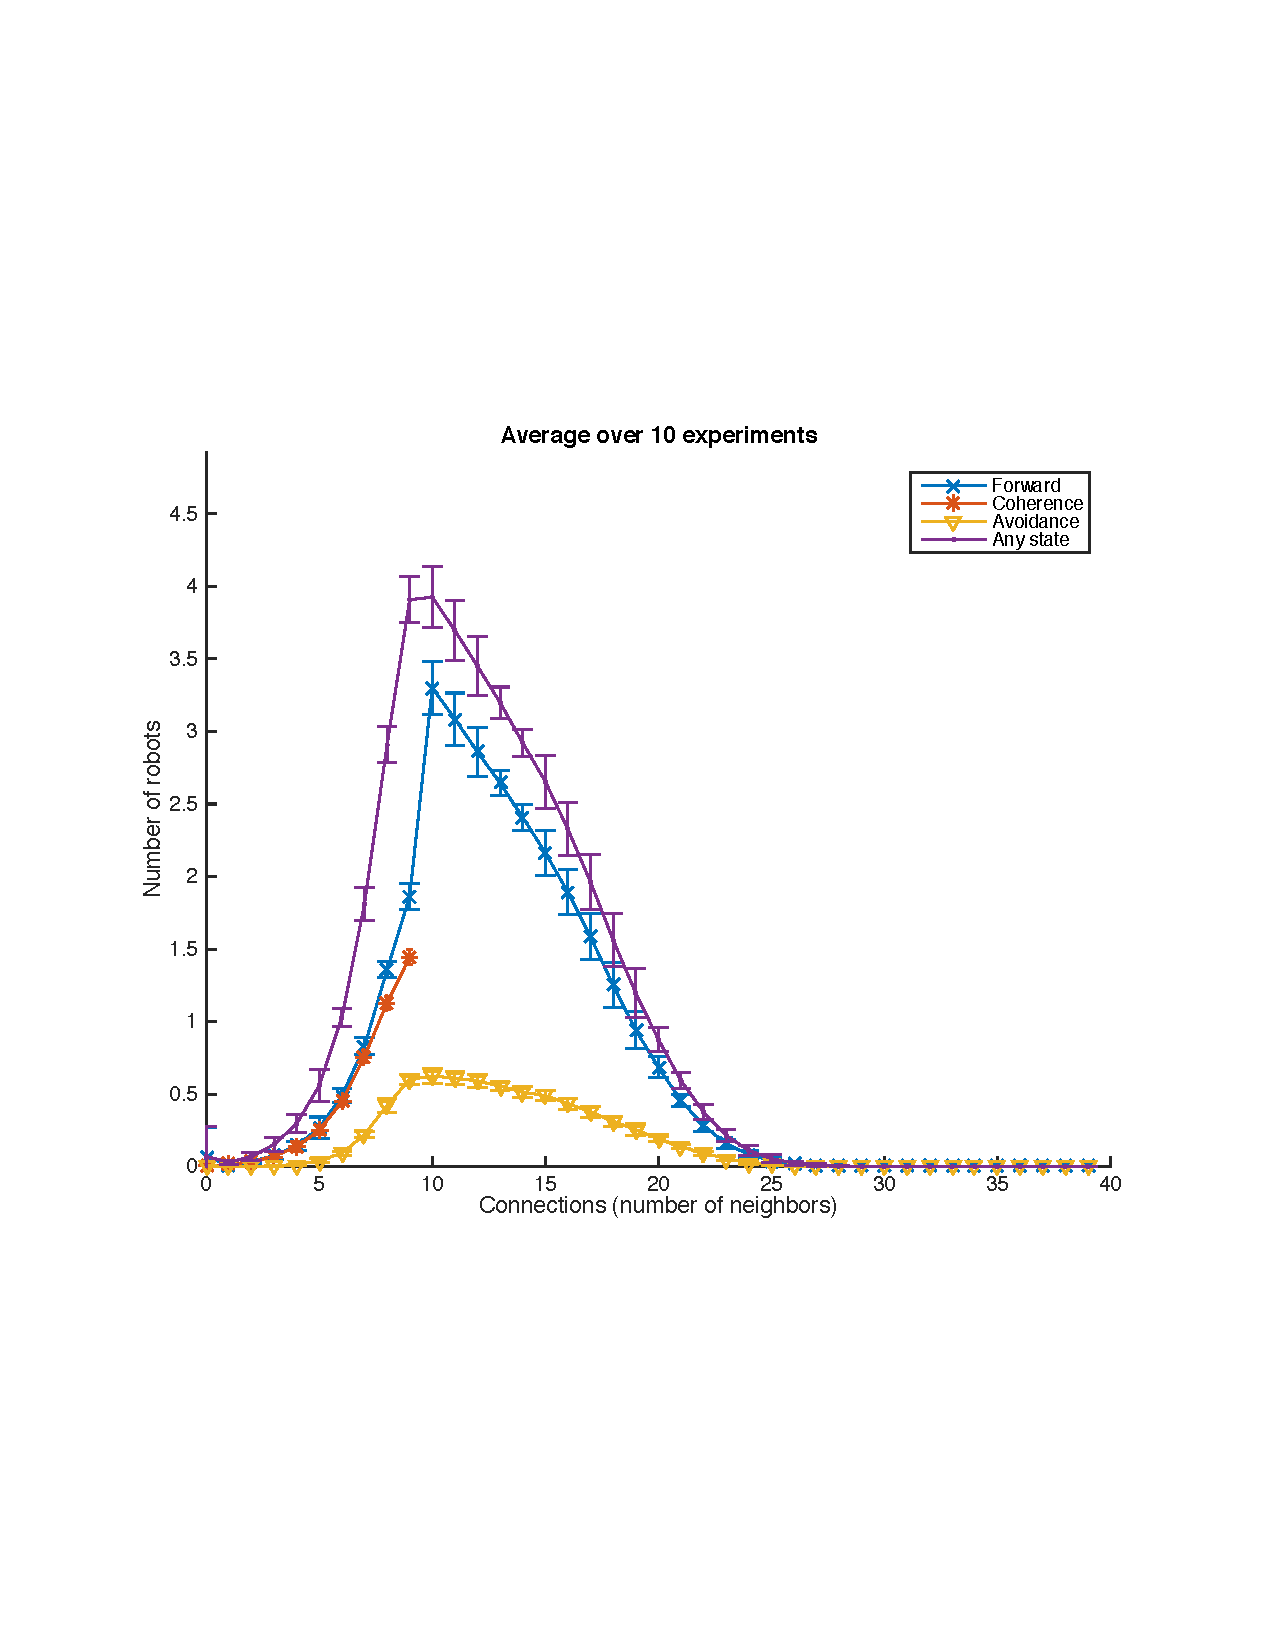
\includegraphics[width=8cm]{figures/simulation-40-alpha10.pdf}
      \caption{TODO: simulation VS macroscopic model for $\alpha = 5$, $10$ and $15$}
    \end{center}
  \end{figure}

  We were able to reproduce the results of \cite{Winfield08}. Compare simulation VS macroscopic.

%%%%%%%%%%%%%%%%%%%%%%%%%%%%%%%%%%%%%%%%%%%%%%%%%%%%%%%%%%%%%%%%%%%%%%%%%%%%%%%%

\section{Conclusion}
  TODO: summary and implications of your findings

%%%%%%%%%%%%%%%%%%%%%%%%%%%%%%%%%%%%%%%%%%%%%%%%%%%%%%%%%%%%%%%%%%%%%%%%%%%%%%%%

%\addtolength{\textheight}{-12cm}  % This command serves to balance the column lengths
                                  % on the last page of the document manually. It shortens
                                  % the textheight of the last page by a suitable amount.
                                  % This command does not take effect until the next page
                                  % so it should come on the page before the last. Make
                                  % sure that you do not shorten the textheight too much.

%%%%%%%%%%%%%%%%%%%%%%%%%%%%%%%%%%%%%%%%%%%%%%%%%%%%%%%%%%%%%%%%%%%%%%%%%%%%%%%%

\begin{thebibliography}{99}

  \bibitem{Nembrini02} Nembrini J, Winfield A and Melhuish C, \textit{Minimalist Coherent Swarming of Wireless Connected Autonomous Mobile Robots}, in Proc. Simulation of Artificial Behaviour '02, Edinburgh, August 2002.

  \bibitem{Winfield08} Winfield AFT, Liu W, Nembrini J and Martinoli A, \textit{Modelling a Wireless Connected Swarm of Mobile Robots}, Swarm Intelligence, 2 (2-4), 241-266, 2008.

\end{thebibliography}

\section*{Acknowledgments}
  TODO

\end{document}
